\section{Electrons}
\label{sec:ch6_electrons}

\subsection{Reconstruction}

The electron object is reconstructed from an ID track matched to an electromagnetic shower in the calorimeter.
Bremsstrahlung photons emitted in the upstream material can spread the shower energy over several clusters and alter the curvature of the electron track.
Both effects are treated in the reconstruction~\cite{ATLAS2019ElectronPerformance}:
\begin{enumerate}
    \item \textbf{Topo-cluster reconstruction.} Neighbouring cells are grouped into topological clusters according to their signal significance above the expected noise. Clusters with a substantial electromagnetic energy fraction are used as electron seeds.
    \item \textbf{Track refitting and matching.} Electron-track candidates are refitted with a Gaussian-sum filter, in which a mixture of Gaussian components is used to describe radiative energy losses. The refitted tracks are extrapolated to the second layer of the EM calorimeter and matched to clusters using their differences in $\eta$ and $\phi$. If several tracks match the same cluster, the $\Delta R$ between each extrapolated track position and the cluster centre is used together with the pixel and SCT hits to rank the tracks.
    \item \textbf{Supercluster formation.} Nearby clusters are added to the seed to recover energy from bremsstrahlung. Additional clusters sharing the matched electron track can be collected over a wider region in $\phi$.
\end{enumerate}
The cluster association is illustrated in Figure~\ref{fig:ch6_electron_supercluster}.
The wider collection in $\phi$ helps recover energy separated from the electron by its bending in the magnetic field.

\begin{figure}[htbp]
    \centering
    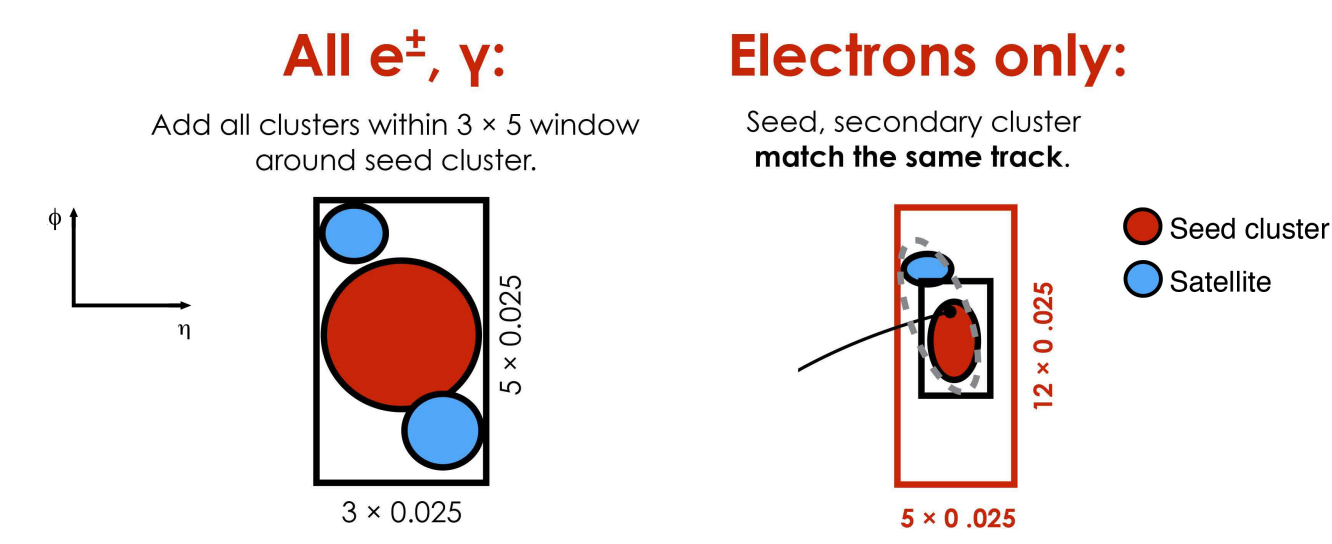
\includegraphics[width=0.75\textwidth]{output/ch6/figures/electron_superclusters.png}
    \caption[Cluster association for electron superclusters]{Cluster association for electron superclusters. Seed and additional clusters are shown in red and blue, respectively. Geometrically nearby clusters are collected~\cite{ATLAS2019ElectronPerformance}.}
    \label{fig:ch6_electron_supercluster}
\end{figure}

\subsection{Identification}

Electron candidates are distinguished from hadronic showers and converted photons using a likelihood discriminant~\cite{ATLAS2019ElectronReco}.
Its inputs include the shower shapes in the EM calorimeter, hit variables, and the agreement between the track and calorimeter measurements.
The \texttt{Loose}, \texttt{Medium} and \texttt{Tight} working points are defined and provide increasing background rejection with the different likelihood discriminant threshold.
The \texttt{Tight} likelihood working point, denoted \texttt{TightLH}, is used for all electron candidates in this analysis.
Its typical prompt-electron identification efficiency is about 80\%~\cite{ATLAS2024ElectronPhotonEfficiencies}.

\subsection{Isolation}

Electrons from hadron decays can pass the electron identification requirements.
These electrons are usually accompanied by other particles from the same jet, while prompt electrons typically have smaller nearby track $\pT$ and calorimeter $\et$ sums.
Isolation requirements are therefore used to suppress this background.

Two isolation variables are calculated using tracks and calorimeter clusters within cones around the electron direction~\cite{ATLAS2019ElectronPerformance}:
\begin{itemize}
    \item \textbf{Track isolation} is performed using the $\pT$ sum of tracks in the cone. At high electron $\pT$, other decay products can lie close to the electron due to the boost effect, so the cone radius is reduced.
    \item \textbf{Calorimeter isolation} follows the same principle as track isolation, but uses cluster $\et$ within a fixed cone of $\Delta R=0.2$. The corrected sum estimates the $\et$ from other particles near the electron~\cite{ATLAS2019ElectronPerformance}.
\end{itemize}
In the analysis, baseline electrons are required to pass \texttt{Loose\_VarRad} isolation while signal electrons must additionally satisfy \texttt{HighPtCaloOnly}.
The \texttt{Loose\_VarRad} working point requires the track and calorimeter isolation sums to be below 15\% and 20\% of the electron $\pT$, respectively.
The \texttt{HighPtCaloOnly} working point requires the calorimeter isolation sum to be below $\max(0.015\,\pT,3.5~\GeV)$~\cite{ATLAS2019ElectronPerformance}.
At high $\et$, the prompt-electron efficiencies are about 99\% for \texttt{Loose\_VarRad} and 90--95\% for \texttt{HighPtCaloOnly}~\cite{ATLAS2024ElectronPhotonEfficiencies}.

\subsection{Calibration}

The electron energy is calibrated for losses in upstream material, energy outside the cluster and variations in detector response~\cite{ATLAS2019ElectronPerformance}.
$\zee$ events are used for the calibration.
Reconstruction, identification and isolation efficiencies are measured with the tag-and-probe method: one electron (the tag) is required to pass strict identification cuts, while the other is used as the probe.
After background subtraction, the efficiency is the fraction of probes that pass the selection.
For a selection efficiency $\epsilon$, the scale factor is defined as
\begin{align}
    \mathrm{SF}=\frac{\epsilon_{\mathrm{data}}}{\epsilon_{\mathrm{MC}}}.
    \label{eq:ch6_efficiency_sf}
\end{align}
The scale factors are then applied to simulated event weights for the electron working points used in this analysis.
